\documentclass{../local}
\begin{document}

\section{REXOS Overall Architecture}
% How we changed the architecture, and why we made which decisions
The initial situation in REXOS is how students in the previous semester left it. Figure 1 shows a overview of all system components.
\begin{figure}[h!]
\flushleft
	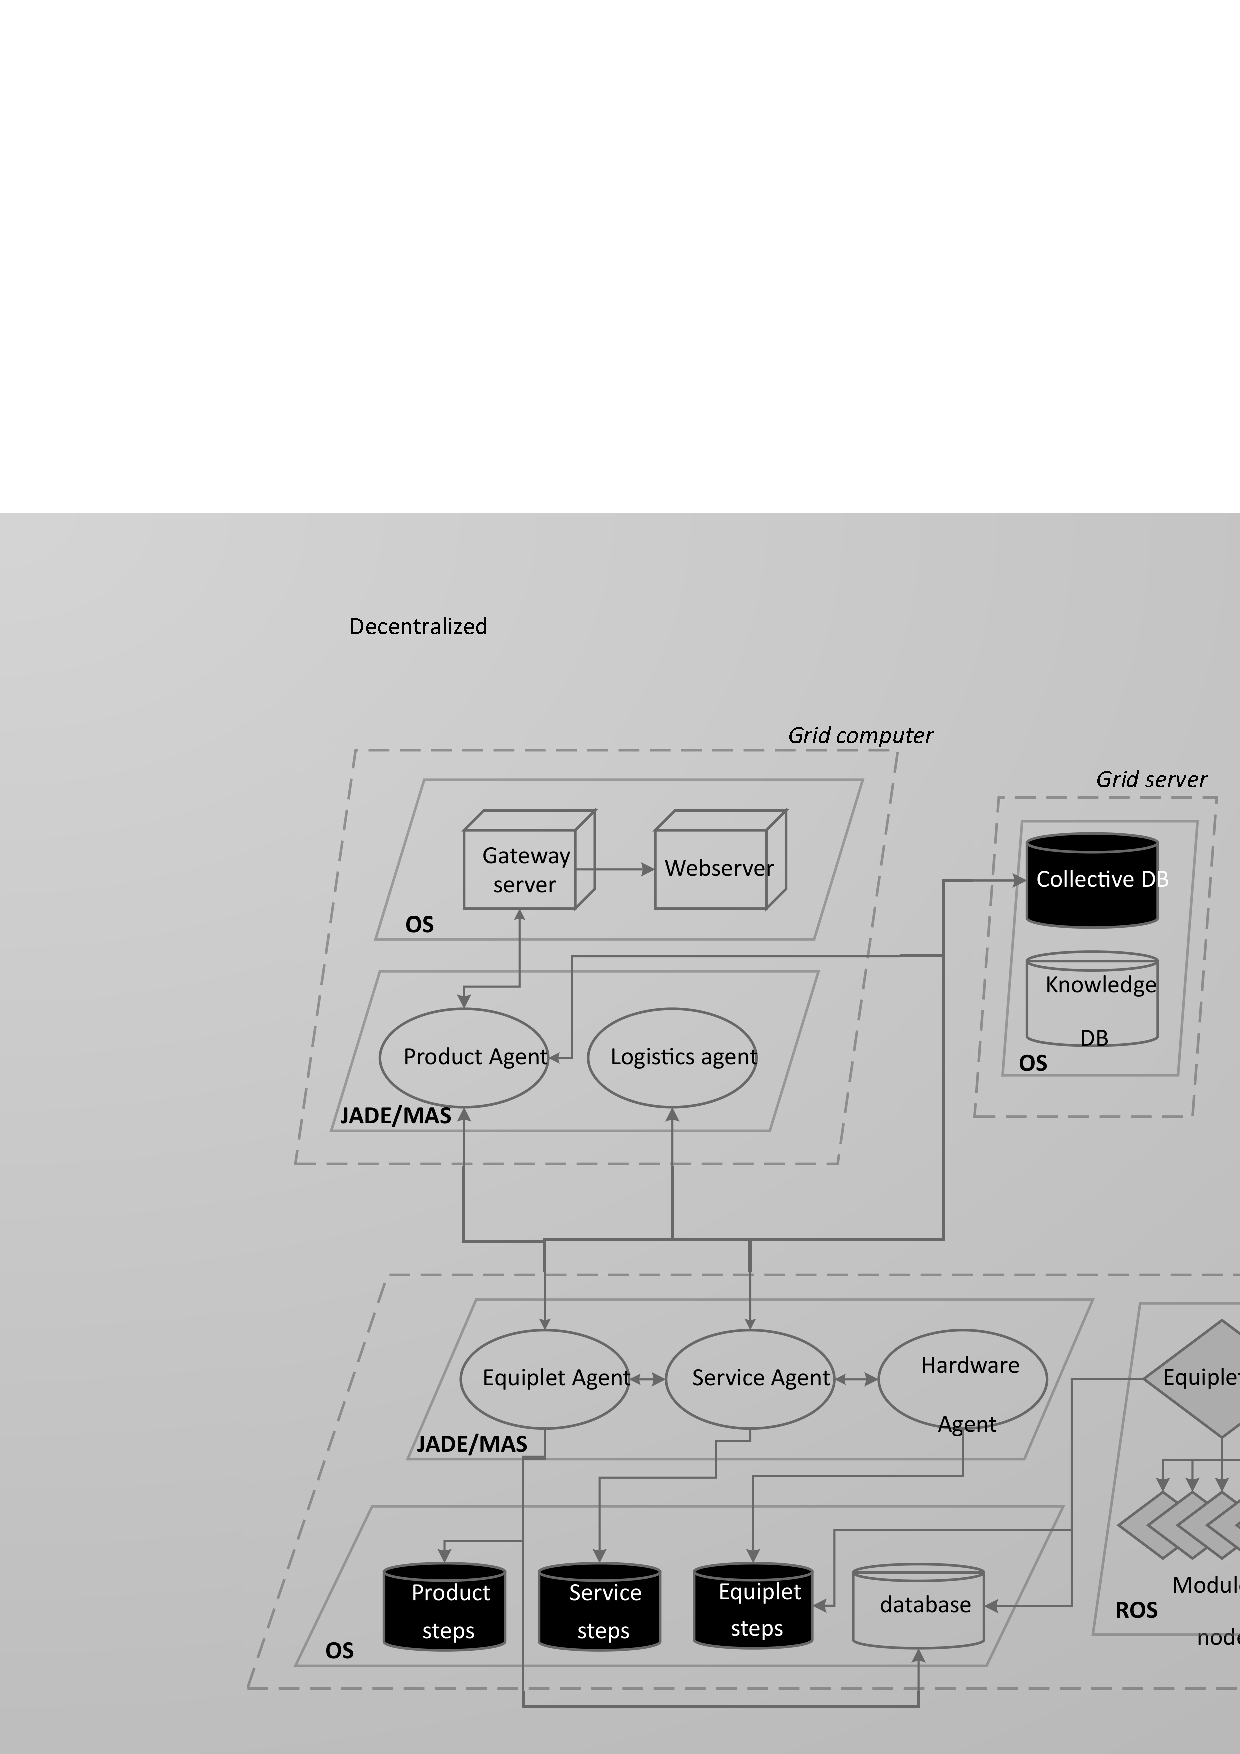
\includegraphics[width=1.1\linewidth]{../images/Decentralized_REXOS.jpg}
	%we might want to increase the text on this image..%
	\caption{System overview}
\end{figure}
When work on REXOS started, the project only functioned in a very limited way. It was designed to give a draw demo, which was far below requirements. The 'mainframe' of the architecture was present, but poorly implemented and documented.
The current system houses 2 major components. MAS, which represents the intellegent part of the system, and ROS, the part responsible for executing commands.

\subsection{MAS}
%Tell smth about implementation of the curr MAS system, what purpose it serves, and how its implemented.%
The MAS\footnote{Multi agent system. See abbreviations for more detail.} was designed to be the intelligent and cognitive side of the the REXOS platform. It incorperates virtual autonomous entities known as agents and is implemented in JADE \textbf{ref2section}. As shown in figure \textbf{ref to system overview} there are currently 5 agents. 

\begin{description}
  \item[Product agent] \hfill \\
		The product agents is a representation of the product. It is responsible for scheduling itself with the equiplets it need for finishing the product it represents.
  \item[Equiplet agent] \hfill \\
  		The equiplet agent is responsible for all communication with the product agent. It handles dealing with its own schedule aswell.
  \item[Service agent] \hfill \\
  		The service agent handles all service level translations. 
  \item[Hardware agent] \hfill \\
  		The hardware agent is responsible for 'controlling' the hardware. It also handles module step translations.
  \item[Logistics agent] \hfill \\
  		The logistics are handles all logistics within a grid. Its responsibilities include providing information about parts.
\end{description}

The MAS also provides a product abstraction. This means that a product 

The current implementation of the MAS is lacking both capability and structure. Previous groups of students have worked on the project and set up the basic version of the MAS. 

\subsubsection{Knowledge database}
The current knowledge database is implemented by the researchers of the previous research-semester. They implemented the knowledge database this way in order to facilitate product abstraction and to provide a central place where data is stored. In this semester realisation came \textbf{realisation came? Really?} that the current implementation is not sufficient enough to facilitate fully autonomous equiplets. 

\subsubsection{New Modules}
In the implementation of REXOS only 1 module was implemented due to time constraints. Due to the nature of the setup of the architecture implementing new modules was required. The modules that are need are modules to allow for pick and placing which include a delta robot module \& a pick and place module.

\subsubsection{Planning}
Another poorly implemented part of the REXOS architecture was the scheduling. the implementation of the schedule didnt take any factors concerning optimisation into account. This is also unimplemented due to time constraints \textbf{ref to document agent projectgroep vorig jaar}.

\subsection{ROS}
%Tell smth about implementation of the curr ROS system, what purpose it serves, and how its implemented.%
The current ROS side of the system represents all the hardware in code. All ROS actions are non-autonomous and driven by the intelligent side of REXOS. This means that all MAS-Agents take smart and cognitive decisions and ROS executes these. 

\subsubsection{Equiplet node}
%het was ruk

\subsubsection{MAST}
% The initial state of MAST
MAST is an abbreviation for MAchine STates and the surrounding system is used for managing the state of the equiplets. The safety and abilities of all systems depend on their internal state. In RMS, having actuators activate when it is not expected can cause harm to people and damage to the surroundings, for that reason, MAST was developed. MAST will insure that an actuator is not activated when it is no expected. It does this using the following model:

\begin{center}
	\includegraphics[width=6cm]{../images/MAST.png}
	\captionof{figure}{The seven states of MAST}
\end{center}

The safe, standby and normal state are active states. The setup, shutdown, start and stop states are transition states. For an entity (equiplet or module) to reach a new active state, it has to successfully traverse the transitional state that precedes it. MAST is setup in such a way that the combined state of all the modules on an equiplet is equal to the highest (furthest from safe) state of any of the modules. This means that if even one module is not in a safe state, the whole equiplet is not safe.

\subsubsection{Vision}
%het was ruk

\subsection{Communication}
Communication between the layers is an important aspect of REXOS. Communication is defined in distinct ways. All data exchange happens through blackboards.A blackboard is a MongoDB implementation with the advantage of allowing read write permissions. This means that blackboards can be configured to allow for one entity to read and write from it, whilst the other is only allowed to write on it. Communication between agents all happends through the JADE ACL(\textbf{ref /  dingen hier}). Communication between ROS and MAS also happends through blackboards.\\
\end{document}